% !TeX root = ../main.tex

\section{Methodology}\label{sec:method}

\begin{figure*}[!t]
  \centering
  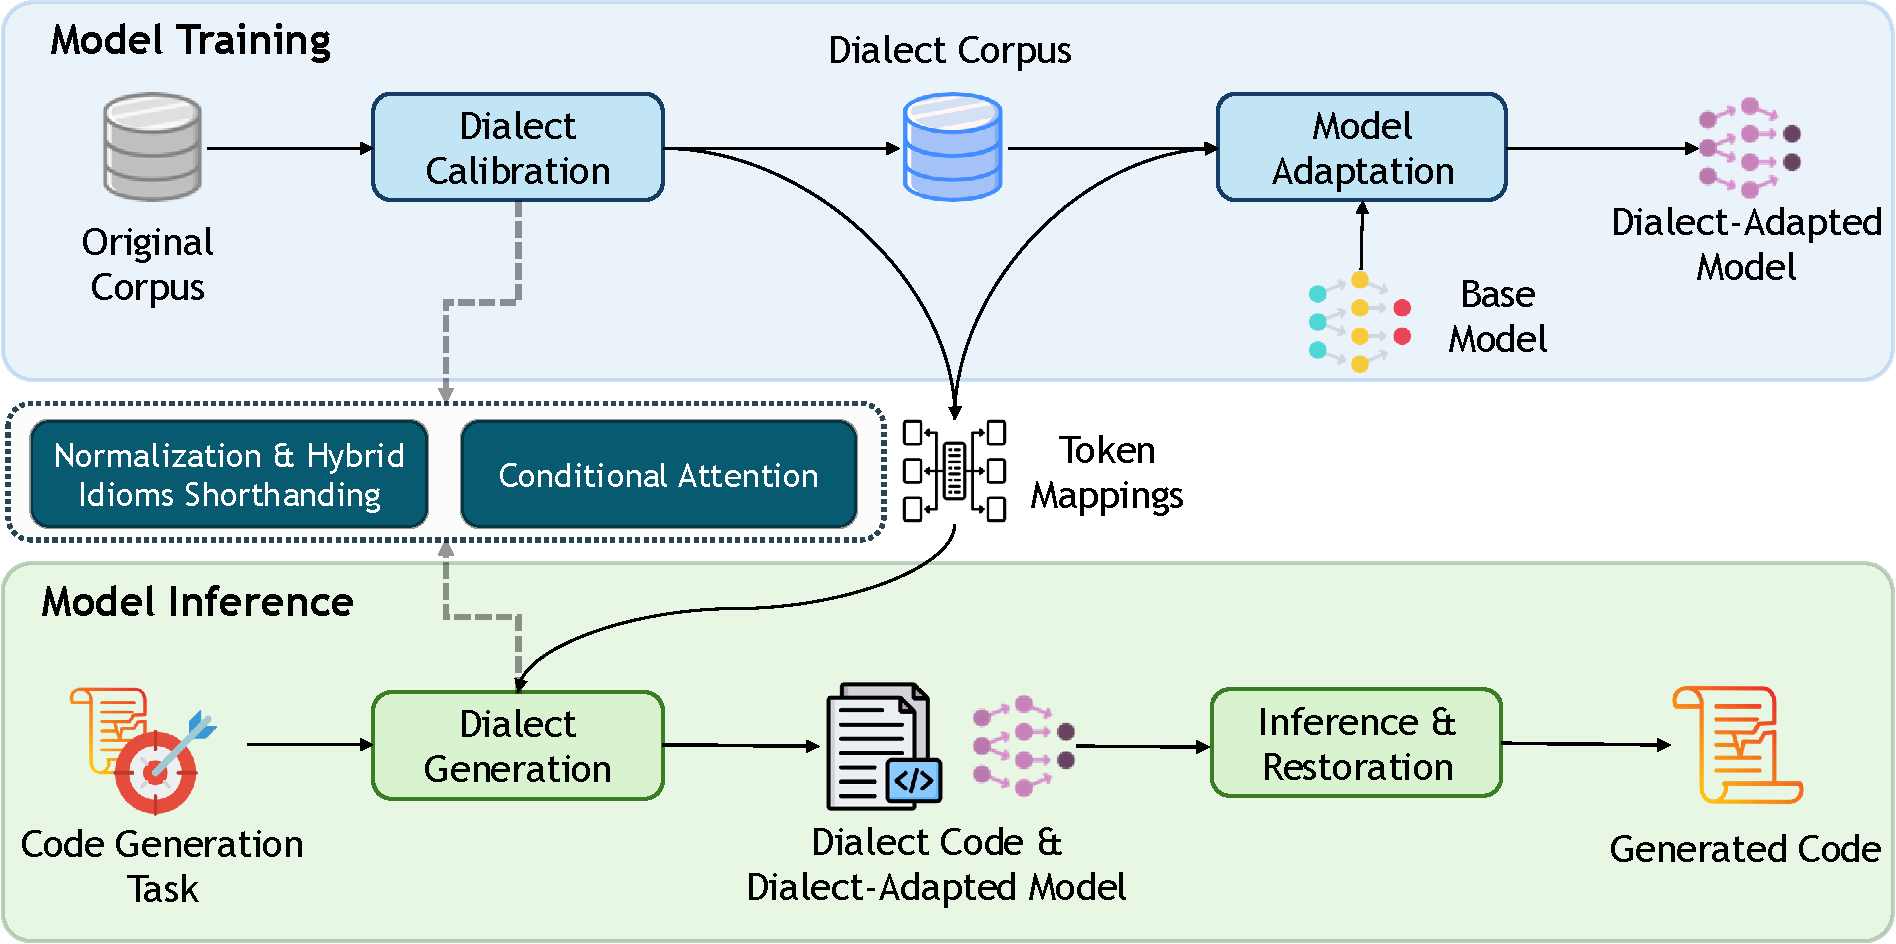
\includegraphics[width=0.8\textwidth]{NormCoRe-2.pdf}
  \vspace{-5pt}
  \caption{Overview of \tool}
  \Description{The NormCoRe workflow contains dialect calibration, model
  adaptation, and dialect-based inference. Calibration applies Normalization,
  Hybrid Idioms Shorthanding, and Conditional Attention; adaptation teaches a
  code model the resulting vocabulary and surface; inference restores generated
  dialect code to ordinary Python.}
  \label{fig:pipeline}
\end{figure*}




This section presents the \tool workflow, from constructing a reversible code dialect to adapting a model and restoring its generated code (Figure~\ref{fig:pipeline}).



\subsection{Overview}

% 介绍一下方法 model training ， model inference， dialect calibration model adaptation, dialect generation等，总体框架

\tool consists of three stages: dialect calibration, model adaptation, and dialect-based inference. Dialect calibration determines how ordinary Python is represented in a shorter but recoverable form. Model adaptation teaches a code model to read and generate that representation. During inference, the adapted model processes the calibrated dialect, and its output is restored to ordinary Python for execution or downstream use.

In \textbf{dialect calibration}, \tool first applies Normalization to compact layout and fixed syntactic structure that can be reconstructed from Python grammar and decoder state. It then collects recurring structures at multiple granularities and represents them through Hybrid Idioms Shorthanding. Fixed and corpus-mined idioms share one registry-based representation, while program-specific identifiers, literals, and expressions are retained directly or carried as captures. Conditional Attention further uses a signal from a reference code model to evaluate eligible shorthand occurrences in context, allowing the calibrated dialect to retain an expanded form where compression would be harder for the model to absorb.

In \textbf{model adaptation}, the shorthand symbols are added to the model vocabulary and the calibrated corpus is used for continued training. The symbols keep stable meanings throughout training, enabling the model to learn both the compact representation and its relationship to ordinary code. This stage turns the dialect from a codec-side transformation into a representation that the model can understand and generate.

In \textbf{dialect-based inference}, source context is encoded with the calibrated \tool representation and supplied to the adapted model. The model may then complete or generate code directly in the dialect. Finally, the reversible decoder expands shorthand symbols, restores normalized structure, and produces ordinary Python. These stages connect token reduction with model training and executable-code generation in one end-to-end workflow.



\subsection{Reversible Shorthanding}
\label{subsec:reversible_mapping}

\tool represents code as a compact textual dialect rather than as a binary compression stream. The dialect remains inside the language model's token space: ordinary program content is kept as code tokens, while recoverable structure and recurring idioms are expressed through a vocabulary of atomic symbols. The model can therefore consume and generate the compressed representation directly.

Let $x$ be a Python program. \tool first applies a deterministic normalization function $N$ that replaces recoverable layout and fixed syntactic structure with structural symbols. It then applies an idiom mapping $Q_{\mathcal{R}}$ defined by a registry $\mathcal{R}$. Each registry entry contains a pattern schema $P_i$, a shorthand symbol $S_i$, and an inverse template. For an occurrence with program-specific captures $c$, the mapping is
\begin{equation}
    P_i(c) \longleftrightarrow \langle S_i, c \rangle,
    \qquad S_i \in \mathcal{V}_{\mathrm{idiom}}.
\end{equation}
The captures carry the identifiers, literals, or expressions needed by that occurrence, so multiple concrete code spans can share one shorthand without discarding their differences. Together, the structural symbols used by $N$ and the idiom symbols used by $Q_{\mathcal{R}}$ form the added dialect vocabulary.

The complete encoder is $E_{\mathcal{R}}=Q_{\mathcal{R}}\circ N$. Its decoder reverses these operations: idiom symbols are expanded with their captures, and the normalized structure is reconstructed from the structural symbols and decoder state. The resulting program preserves the original syntax tree:
\begin{equation}
    \operatorname{AST}\!\left(D_{\mathcal{R}}(E_{\mathcal{R}}(x))\right)
    = \operatorname{AST}(x).
\end{equation}
This formulation provides a common reversible representation for both structural normalization and idiom shorthanding. The following subsections explain how \tool constructs this representation and how Conditional Attention decides where eligible idioms are materialized.

\subsection{Dialect Calibration and Generation}

\subsubsection{Normalization \& Hybrid Idioms Shorthanding}
\label{subsec:codec}

Dialect calibration constructs the representation that will be shared by the training corpus and the adapted model. \tool first applies Normalization to the input program. Guided by Python's concrete syntax and decoder state, it replaces recoverable indentation, line organization, block boundaries, and selected fixed syntax with structural symbols. Program-specific identifiers, literals, and expressions remain explicit. Besides reducing structural tokens directly, this step maps stylistically different programs onto a more regular surface for idiom collection.

Hybrid Idioms Shorthanding then collects recurring structures from the normalized corpus. The collector considers contiguous local windows and syntax-derived expression or statement spans, allowing it to represent idioms at multiple granularities. Exact patterns retain fully shared content, while generalized patterns replace varying identifiers, literals, or expressions with typed captures. Each selected schema is assigned an atomic shorthand symbol and an inverse template in the registry.

Pattern utility is measured on the complete shorthand representation under the target tokenizer, rather than by corpus frequency alone. For an occurrence $m$ of pattern $p$, let $z_m$ be its normalized span and let $g_p(c_m)$ contain the shorthand symbol and captures $c_m$. Its token saving is
\begin{equation}
    \Delta(m)=|T(z_m)|-|T(g_p(c_m))|,
\end{equation}
where $T$ is the target tokenizer. Occurrences with non-positive saving are discarded. The resulting registry therefore concentrates on idioms whose symbols still save tokens after their capture content is included.

Candidate occurrences may overlap. \tool treats them as weighted intervals and uses dynamic programming to select a non-overlapping set with maximum total saving:
\begin{equation}
    S^*=\arg\max_{S\ \mathrm{nonoverlap}}
    \sum_{m\in S}\Delta(m).
\end{equation}
The selected occurrences are materialized on the normalized surface using their shorthand symbols and captures. In this sense, dialect generation is an offline corpus transformation: it creates the compact code seen during model adaptation rather than adding another operation to autoregressive decoding.

Figure~\ref{fig:compression_examples} uses four labels for the granularities of
the mined examples. ``Layout and Structure'' denotes formatting and fixed
structural syntax that Normalization can reconstruct from grammar and decoder
state. ``Function Skeleton'' denotes a recurring function-definition shape
whose identifiers or expressions may vary. ``Multi-statement Span'' denotes a
contiguous recurring sequence containing more than one statement. ``Expression
and Call'' denotes a recurring expression-level or method-call idiom. In the
figure, ``Normalization'' is the normalized intermediate surface and ``Hybrid
Idioms'' is the shorthand surface in which registry symbols and typed captures
are materialized. These labels describe the scope of each example, not
additional compression algorithms.

\begin{figure*}[!t]
  \centering
  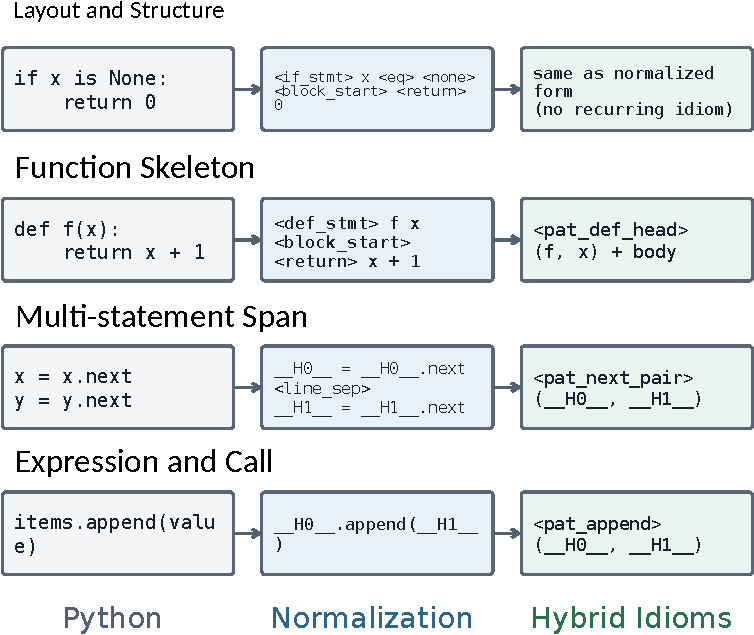
\includegraphics[width=0.7\textwidth]{NormCoRe_compression_examples_terms_cropped.pdf}
  \vspace{-5pt}
  \caption{Representative transformations in \tool. Normalization compacts recoverable layout and syntax, while Hybrid Idioms Shorthanding replaces recurring structures with registry symbols and typed captures. Program-specific content remains explicit or is carried by the captures.}
  \Description{Four examples show Python code transformed into a normalized structural dialect and then, where applicable, into a registry pattern with captures. The examples cover layout, function skeletons, multi-statement spans, and expressions or calls.}
  \label{fig:compression_examples}
\end{figure*}

\subsubsection{Conditional Attention}
\label{subsec:conditional_attention}

Not every legal occurrence of a shorthand imposes the same representation cost on a code model. The same idiom may appear in different control-flow and prediction contexts, and uniformly replacing every match ignores these differences. Conditional Attention therefore evaluates eligible occurrences individually while leaving the normalization rules, shorthand registry, and decoder unchanged.

For each occurrence $m$, \tool considers its expanded normalized context and a counterfactual context in which only that occurrence is replaced. A frozen reference model produces a contextual attention profile that summarizes how attention is allocated around the occurrence and how that allocation changes after replacement. This profile captures both the local importance of the original span and the response of its surrounding prediction context to the shorthand. We denote its standardized representation by $\mathbf{z}(m)$.

The contextual profile is calibrated against the local representation shift caused by the replacement. Let $y_m$ be a common suffix following the occurrence. We measure the change in its mean negative log-likelihood as
\begin{equation}
    d(m)=\operatorname{NLL}_{\mathcal{M}}(y_m\mid x_m^{\mathrm{short}})
         -\operatorname{NLL}_{\mathcal{M}}(y_m\mid x_m^{\mathrm{expanded}}).
\end{equation}
A positive value indicates that the shorthand makes the unchanged continuation harder for the reference model to predict. On a calibration split, \tool fits a regularized linear scorer
\begin{equation}
    \widehat d(m)=b+\mathbf{w}^{\top}\mathbf{z}(m)
\end{equation}
and then keeps the scorer fixed when constructing training or evaluation dialects.

To materialize a dialect at a chosen reduction level, eligible occurrences are ordered from the lowest to the highest predicted damage and admitted until the target number of token removals is reached. The admitted occurrences then enter the same non-overlapping selection used by Hybrid Idioms Shorthanding. Because the decision is occurrence-specific, two instances of the same registry pattern may be represented differently when their contexts produce different model responses. Conditional Attention is applied offline during dialect construction; it does not require an additional attention computation during model generation.

\subsection{Model Adaptation}

After dialect calibration, the structural symbols introduced by Normalization and the idiom symbols registered by Hybrid Idioms Shorthanding are added to the model vocabulary as atomic tokens. Source programs are transformed with the calibrated encoder, including the occurrence decisions made by Conditional Attention, to construct the dialect corpus used for adaptation. The meanings of these symbols remain consistent across the corpus: a structural symbol always represents the same recoverable syntax, and an idiom symbol always invokes the same registry schema and inverse template.

\tool adapts the model with the standard autoregressive language-modeling objective. For a materialized dialect sequence $\widetilde{x}=E_{\mathcal{R}}(x)$, the objective is
\begin{equation}
    \mathcal{L}_{\mathrm{adapt}}
    =-\sum_{t=1}^{|\widetilde{x}|}
    \log p_{\theta}(\widetilde{x}_t\mid \widetilde{x}_{<t}).
\end{equation}
No change to the model architecture or generation objective is required. Through continued training, the model learns how the added symbols interact with ordinary code tokens, how structural markers organize a program, and how shorthand symbols represent recurring code idioms. For symmetric dialect generation, both the context and target code use the \tool representation. When native output is preferred, the model can instead receive a condensed context while being supervised on ordinary Python targets.

\subsection{Inference and Restoration}

During dialect-based inference, the available source context is transformed with the same calibrated encoder used to prepare the training corpus. The adapted model then reads the shortened context and generates either \tool dialect code or native Python, according to the adaptation setting. Conditional Attention is part of dialect preparation and does not alter the model's autoregressive generation procedure.

For dialect output, restoration reverses the encoding stages in order. The decoder first expands each idiom symbol with its accompanying captures according to the registry template. It then restores the layout and fixed syntactic structure represented by the normalization symbols. The resulting ordinary Python program can be passed directly to existing parsers, execution environments, and software-engineering tools. In this way, token reduction remains internal to the model-facing representation, while the external interface continues to use standard source code.
